% Generated by robotic_arm_analysis/make_figures.py -- data source: offline
% Requires: graphicx, booktabs, tabularx, float, cleveref.  Images in images/sim/.
\subsection{Motion and kinematics (Gazebo)}
The SolidWorks assembly is exported to URDF and cleaned (joint limits, upright mounting, J4/J5 names, collision hulls); the same file
feeds the Gazebo model and the calculations of this section. The results below come from an offline rigid-body simulation of the same URDF (articulated-body dynamics, 1~ms step), with the joint torque limits of
\cref{tab:simtorque}, the planned joint speed of 60\textdegree/s and a payload of
50~g. The sequence is the one of the real arm: homing of J1 to J4 on limit switches, then
approach, descend, grasp, lift, classify, move to bin, release and return, for 4 objects of two colours.

\IfFileExists{images/sim/gazebo_arm.png}{%
\begin{figure}[H]
  \centering
  \includegraphics[width=0.85\linewidth]{images/sim/gazebo_arm.png}
  \caption{Gazebo model of the arm during a pick.}
  \label{fig:simgazebo}
\end{figure}}{}

The inverse kinematics are solved numerically (damped least squares on the URDF chain). One arm configuration and one tool
orientation, tilted 10\textdegree{} from the vertical, are kept for the whole cycle, so the elbow never flips. All
6 targets are reached, and the rigid-body simulation follows the trapezoidal joint profiles with a largest tracking error of
0.36\textdegree{} (\cref{fig:simangles}). One pick-and-place cycle takes 13.6~s.
Homing takes 11.8~s; each joint stops within 0.01\textdegree{} of its switch at a seek speed of
8\textdegree/s (\cref{fig:simhoming}).

\begin{figure}[H]
  \centering
  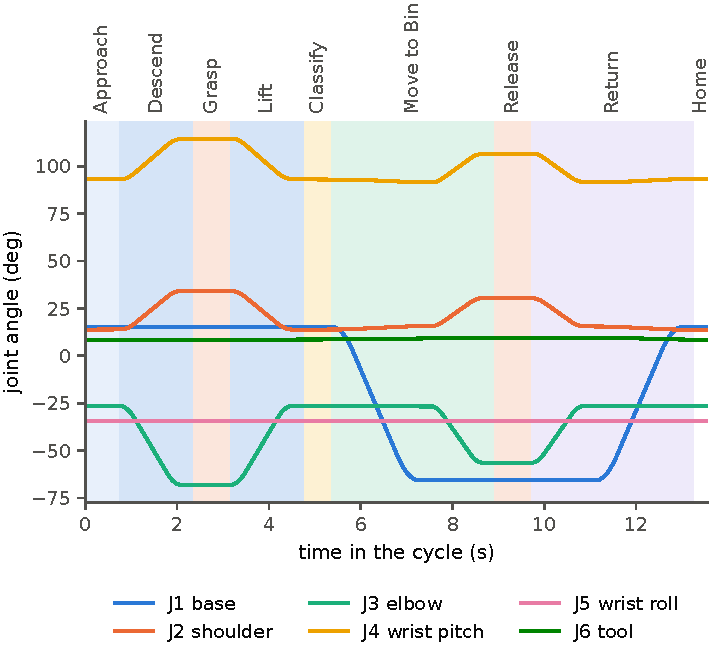
\includegraphics[width=0.85\linewidth]{images/sim/sim_joint_angles.pdf}
  \caption{Joint angles over one pick-and-place cycle; the shaded bands are the states of the sequence.}
  \label{fig:simangles}
\end{figure}

\begin{figure}[H]
  \centering
  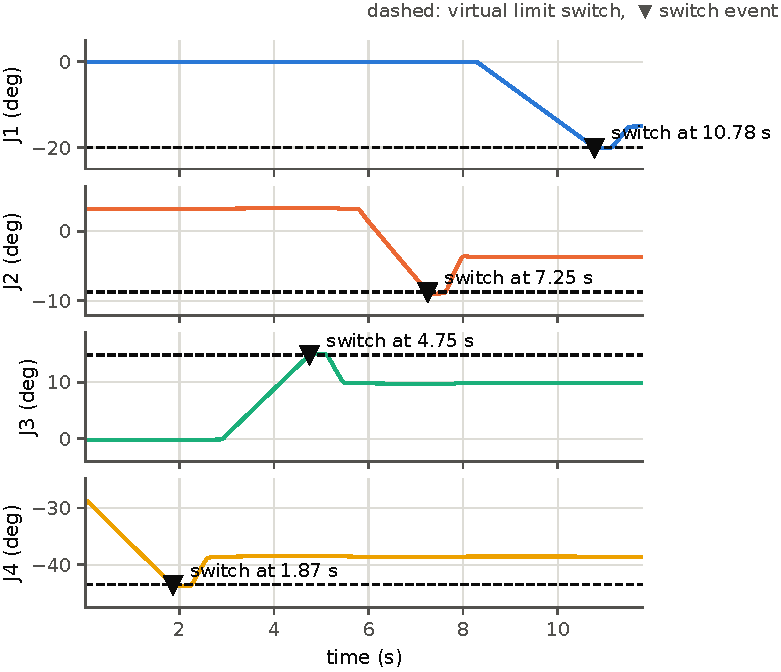
\includegraphics[width=0.85\linewidth]{images/sim/sim_homing.pdf}
  \caption{Homing of J4 to J1: each joint seeks its limit switch, stops, backs off and sets its zero.}
  \label{fig:simhoming}
\end{figure}

The tool centre point reaches 746~mm from the J1 axis (\cref{fig:simworkspace}). With this tool orientation,
the torque rule of \cref{tab:simtorque} is met only in a band between 120 and
240~mm radius and not at table height; with the tool folded closer to the upper arm the torque is lower, but the links come within 15~mm of each other. This fixes the layout: the pick location is a stand
185~mm high at 200~mm radius, and the two bins
are raised to a rim height of 180~mm at 210~mm radius, 80\textdegree{}
on either side of the pick location.

\begin{figure}[H]
  \centering
  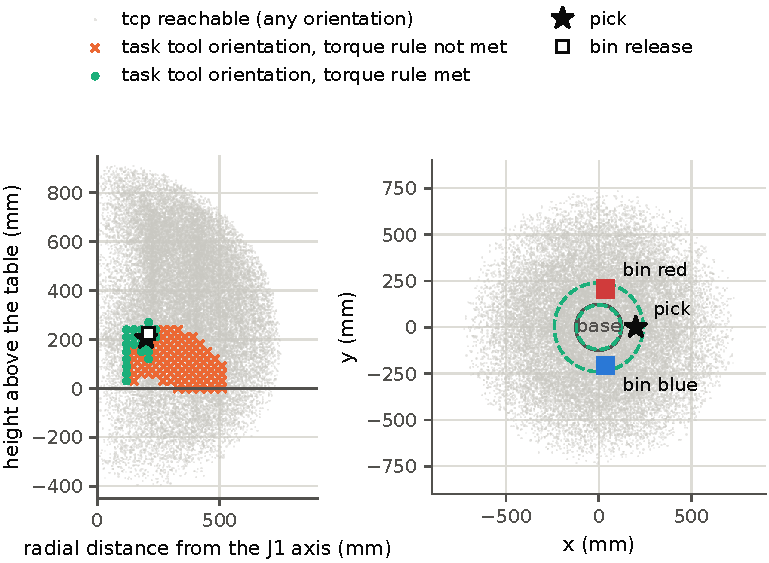
\includegraphics[width=0.85\linewidth]{images/sim/sim_workspace.pdf}
  \caption{Reachable workspace of the tool centre point: side view (left) and top view (right), with the pick location and the bins.}
  \label{fig:simworkspace}
\end{figure}

\subsection{Clearance}
The distance between the arm and its surroundings is computed along the simulated path from the CAD meshes of the links, the jaws
and the carried object, with a resolution of about 3~mm. The smallest distance is 145~mm to the table,
8~mm to the pick stand and the bins (state lift), and
35~mm between links that are not neighbours (\cref{fig:simclearance}); two pairs joined through a short link,
which are 16 to 34~mm apart by construction, are left out.
No collision occurs.
The travel height of 260~mm is kept, which leaves
65~mm between the carried
object and the rim of the bins.

\begin{figure}[H]
  \centering
  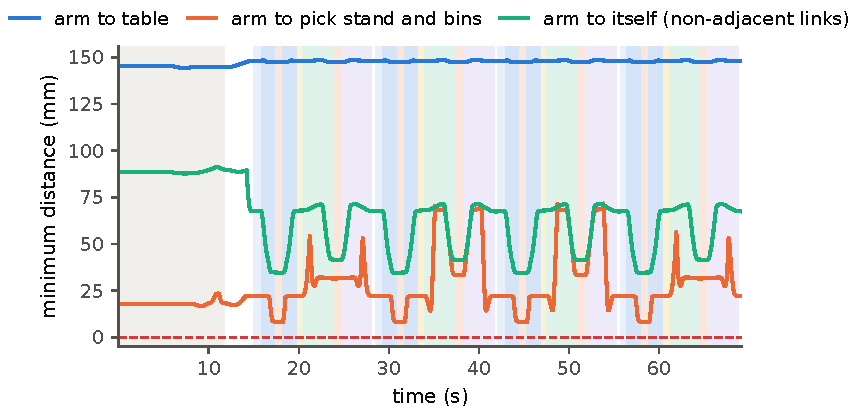
\includegraphics[width=0.85\linewidth]{images/sim/sim_clearance.pdf}
  \caption{Minimum distance from the arm to the table, to the pick stand and bins, and to itself along the sequence.}
  \label{fig:simclearance}
\end{figure}

\subsection{Torque and load}
The static torque of each joint is computed from the URDF masses (2.37~kg beyond J2, payload included) as the gravity
torque of everything beyond the joint. \Cref{tab:simtorque} gives it for the worst pose inside the joint range and for the worst pose
of the pick-and-place task, with the factor 1.5 for acceleration. The gripper row is the servo torque that holds the object by friction
(coefficient 0.5, pinion radius 10~mm).

\begin{table}[H]
  \centering
  \caption{Torque check per joint. Required $=1.5\times$ static; margin $=$ available$/$required.}
  \label{tab:simtorque}
  \begin{tabularx}{\linewidth}{l X r r r r r r}
    \toprule
     & & & \multicolumn{3}{c}{Worst pose in range} & \multicolumn{2}{c}{Task poses} \\
    \cmidrule(lr){4-6}\cmidrule(lr){7-8}
    Joint & Actuator & Available & Static & Required & Margin & Static & Margin \\
     & & (N\,m) & (N\,m) & (N\,m) & & (N\,m) & \\
    \midrule
    J2 shoulder & 17HS4401 $+$ 1:14 & 3.90 & 8.37 & 12.56 & 0.31 & 1.86 & 1.40 \\
    J3 elbow & 17HS4401 $+$ 1:14 & 3.90 & 4.21 & 6.31 & 0.62 & 0.63 & 4.15 \\
    J4 wrist pitch & 17HS4401 $+$ 1:14 & 3.90 & 1.45 & 2.18 & 1.79 & 1.30 & 2.00 \\
    J5 wrist roll & DS3218MG & 1.96 & 0.81 & 1.21 & 1.62 & 0.10 & 13.14 \\
    J6 tool & DS3218MG & 1.96 & 0.002 & 0.003 & $>$ 100 & 0.000 & $>$ 100 \\
    Gripper & MG996R & 1.08 & 0.005 & 0.007 & $>$ 100 & 0.005 & $>$ 100 \\
    \bottomrule
  \end{tabularx}
\end{table}

With the arm stretched out horizontally, J2 would need 12.6~N\,m and J3 6.3~N\,m,
against 3.9~N\,m available: the margins are 0.31 and 0.62, so
the arm cannot work at full reach. Inside the task envelope the margins are 1.40 for J2,
4.15 for J3 and 2.00 for J4. Along the simulated cycles the peak torques are
2.19~N\,m on J2, 0.97~N\,m on J3 and 1.70~N\,m on J4, that is
56~\% of the available torque at most (\cref{fig:simtorques}). The decision is to keep the
17HS4401 and the 1:14 reducer and to restrict the work to the raised stations close to the base; working at full reach would need a
reduction of about 1:45 on J2 and 1:23 on J3, or lighter links.

\begin{figure}[H]
  \centering
  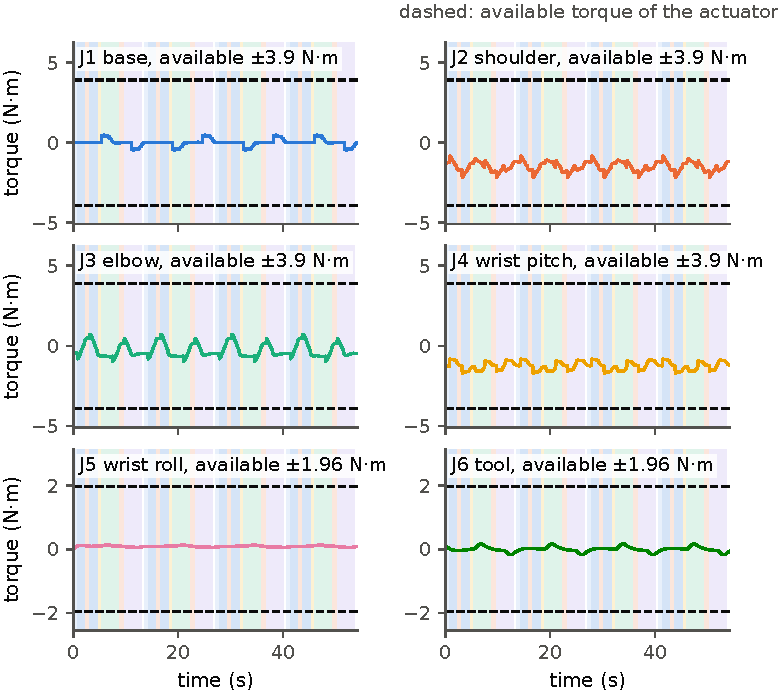
\includegraphics[width=0.85\linewidth]{images/sim/sim_joint_torques.pdf}
  \caption{Joint torques over 4 pick-and-place cycles, compared with the available torque of each actuator.}
  \label{fig:simtorques}
\end{figure}

\subsection{Power and control logic}
The mechanical power of each stepper joint is the product of torque and joint speed. Its peak over the cycles is
0.73~W (J2), below the 9.4~W assumed per joint in the power
budget (\cref{fig:simpower}); the budget is therefore conservative for this task.

\begin{figure}[H]
  \centering
  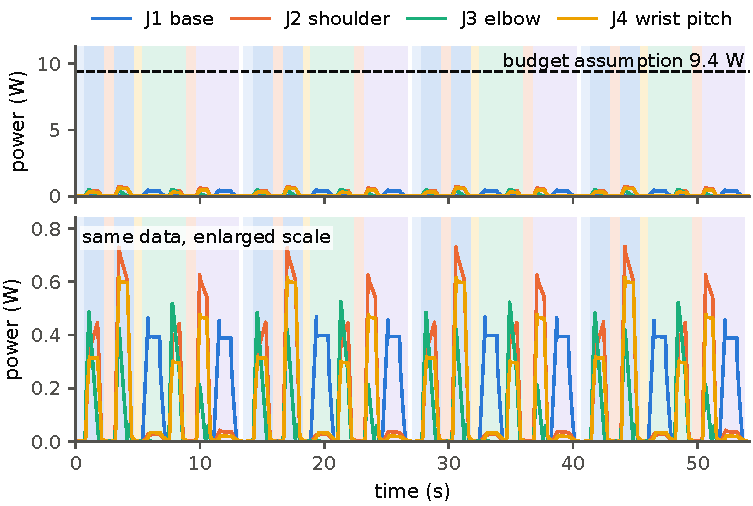
\includegraphics[width=0.85\linewidth]{images/sim/sim_power.pdf}
  \caption{Mechanical power of the stepper joints over the cycles, compared with the power budget assumption.}
  \label{fig:simpower}
\end{figure}

The emergency stop was tested while the arm holds the payload at the travel height: the torque of J1 to J4 is set to zero, as the hardware does by disabling the drivers, and the servos stay powered (\cref{fig:simestop}). With the assumed unpowered friction of 0.3~N\,m at the joint (motor detent torque through the 1:14 reducer), the static load of 1.86~N\,m on J2 is not held: J2 moves by 57\textdegree{} and J3 by 2\textdegree. The tool reaches the pick stand 0.49~s after the stop. The risk ``joints drop when the E-stop removes torque'' is therefore confirmed: the reducer does not hold the arm unless its unpowered friction exceeds 1.9~N\,m, which has to be measured on the first printed gearbox. The rule that nobody stands near the arm during tests is kept, and the pick stand stops the fall of the tool.

\IfFileExists{images/sim/sim_estop.pdf}{%
\begin{figure}[H]
  \centering
  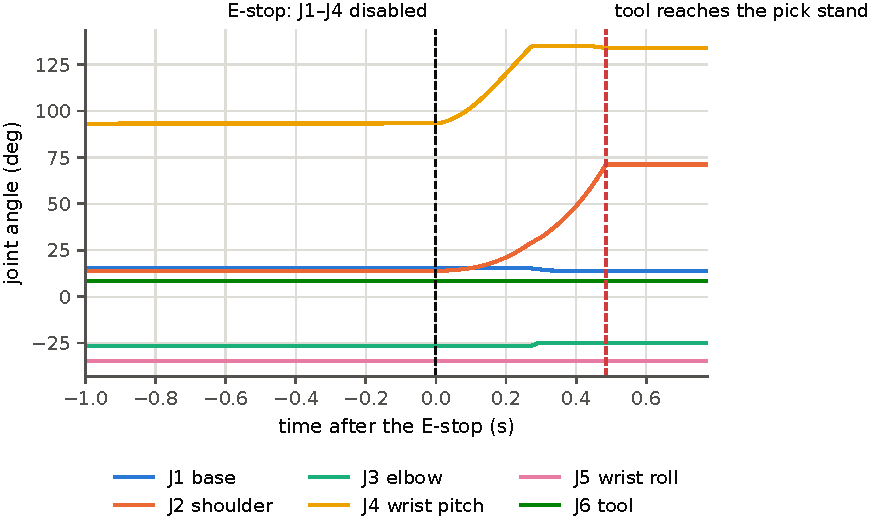
\includegraphics[width=0.85\linewidth]{images/sim/sim_estop.pdf}
  \caption{Joint angles after the emergency stop removes the torque of J1 to J4.}
  \label{fig:simestop}
\end{figure}}{}
